%%
%% This is file `sample-sigconf.tex',
%% generated with the docstrip utility.
%%
%% The original source files were:
%%
%% samples.dtx  (with options: `sigconf')
%%
%% IMPORTANT NOTICE:
%%
%%% For the copyright see the source file.
%%
%% Any modified versions of this file must be renamed
%% with new filenames distinct from sample-sigconf.tex.
%%
%% For distribution of the original source see the terms
%% for copying and modification in the file samples.dtx.
%%
%% This generated file may be distributed as long as the
%% original source files, as listed above, are part of the
%% same distribution. (The sources need not necessarily be
%% in the same archive or directory.)
%%
%% The first command in your LaTeX source must be the \documentclass command.

% Modify this to remove all ACM and conference information (for arXiv for example)
\def\removeHeaders{yes}



\def\tempYes{yes}
\documentclass[9pt,sigconf,letterpaper,dvipsnames\ifx\removeHeaders\tempYes ,nonacm\fi]{acmart}

\copyrightyear{2019}
\acmYear{2019}
\setcopyright{acmcopyright}
\acmConference[Big-DAMA '19]{3rd ACM CoNEXT Workshop on Big DAta, Machine Learning and Artificial Intelligence for Data Communication Networks}{December 9, 2019}{Orlando, FL, USA}
\acmBooktitle{3rd ACM CoNEXT Workshop on Big DAta, Machine Learning and Artificial Intelligence for Data Communication Networks (Big-DAMA '19), December 9, 2019, Orlando, FL, USA}
\acmPrice{15.00}
\acmDOI{10.1145/3359992.3366638}
\acmISBN{978-1-4503-6999-2/19/12}

\usepackage[utf8]{inputenc}

\usepackage{multirow}
\usepackage{blindtext}
\usepackage{soul}
\usepackage[inline]{enumitem}

\usepackage{subfig}

% Acronyms
\usepackage[nomain, toc, acronym]{glossaries}
\glsdisablehyper

\ifx\removeHeaders\tempYes
\settopmatter{printacmref=false} % Removes citation information below abstract
\renewcommand\footnotetextcopyrightpermission[1]{} % removes footnote with conference information in first column
\fi

\newcommand\note[2]{{\color{#1}#2}}
\newcommand\todo[1]{{\note{red}{TODO: #1}}}

\newcommand{\unsw}{UNSW-NB15}
\newcommand{\cic}{CIC-IDS-2017}

%%
%% \BibTeX command to typeset BibTeX logo in the docs
\AtBeginDocument{%
  \providecommand\BibTeX{{%
    \normalfont B\kern-0.5em{\scshape i\kern-0.25em b}\kern-0.8em\TeX}}}


%%
%% Submission ID.
%% Use this when submitting an article to a sponsored event. You'll
%% receive a unique submission ID from the organizers
%% of the event, and this ID should be used as the parameter to this command.
%%\acmSubmissionID{123-A56-BU3}

%%
%% The majority of ACM publications use numbered citations and
%% references.  The command \citestyle{authoryear} switches to the
%% "author year" style.
%%
%% If you are preparing content for an event
%% sponsored by ACM SIGGRAPH, you must use the "author year" style of
%% citations and references.
%% Uncommenting
%% the next command will enable that style.
%%\citestyle{acmauthoryear}

%%
%% end of the preamble, start of the body of the document source.
\begin{document}

%%
%% The "title" command has an optional parameter,
%% allowing the author to define a "short title" to be used in page headers.
\title{Eager-Stopping: Early Network Intrusion Prediction\\in Feed Forward Neural Networks}

%% GLOSSARY

\newacronym{dl}{DL}{Deep Learning}
\newacronym{ad}{AD}{Anomaly Detection}
\newacronym{ml}{ML}{Machine Learning}
\newacronym{ttl}{TTL}{Time-to-Live}
\newacronym{ids}{IDS}{Intrusion Detection System}
\newacronym{mlp}{MLP}{Multilayer Perceptron}
\newacronym{relu}{ReLU}{Rectified Linear Unit}
\newacronym{ip}{IP}{Internet Protocol}

\begin{abstract}
	
\end{abstract}

\ifx\removeHeaders\tempNo
	\begin{CCSXML}
		<ccs2012>
		<concept>
		<concept_id>10002978.10002997.10002999</concept_id>
		<concept_desc>Security and privacy~Intrusion detection systems</concept_desc>
		<concept_significance>500</concept_significance>
		</concept>
		<concept>
		<concept_id>10010147.10010257.10010293.10003660</concept_id>
		<concept_desc>Computing methodologies~Classification and regression trees</concept_desc>
		<concept_significance>500</concept_significance>
		</concept>
		<concept>
		<concept_id>10010147.10010257.10010293.10010294</concept_id>
		<concept_desc>Computing methodologies~Neural networks</concept_desc>
		<concept_significance>500</concept_significance>
		</concept>
		<concept>
		<concept_id>10003033.10003083.10003014</concept_id>
		<concept_desc>Networks~Network security</concept_desc>
		<concept_significance>300</concept_significance>
		</concept>
		</ccs2012>
	\end{CCSXML}
	\ccsdesc[500]{Security and privacy~Intrusion detection systems}
	\ccsdesc[500]{Computing methodologies~Classification and regression trees}
	\ccsdesc[500]{Computing methodologies~Neural networks}
	\ccsdesc[300]{Networks~Network security}
	\keywords{Network security, Deep Learning, }
\fi

%%
%% The "author" command and its associated commands are used to define
%% the authors and their affiliations.
%% Of note is the shared affiliation of the first two authors, and the
%% "authornote" and "authornotemark" commands
%% used to denote shared contribution to the research.

%\author{Maximilian Bachl, Alexander Hartl, Joachim Fabini, Tanja Zseby}
%\affiliation{\institution{Technische Universität Wien}}
%\email{firstname.lastname@tuwien.ac.at}


%%
%% By default, the full list of authors will be used in the page
%% headers. Often, this list is too long, and will overlap
%% other information printed in the page headers. This command allows
%% the author to define a more concise list
%% of authors' names for this purpose.
%\renewcommand{\shortauthors}{Hartl and Bachl}

%%
%% The abstract is a short summary of the work to be presented in the
%% article.
%\begin{abstract}
%  A clear and well-documented \LaTeX\ document is presented as an
%  article formatted for publication by ACM in a conference proceedings
%  or journal publication. Based on the ``acmart'' document class, this
%  article presents and explains many of the common variations, as well
%  as many of the formatting elements an author may use in the
%  preparation of the documentation of their work.
%\end{abstract}
\ifx\removeHeaders\tempYes
	\settopmatter{printfolios=true}
\fi
\maketitle



\section{Introduction}

\section{Supervised Learning for Network Intrusion Detection}

\section{Eager-Stopping}
\subsection{Feed Forward Neural Networks}

\subsection{Early Predictions}

\begin{figure*}[htp]

\subfloat[Conventional Feed Forward Neural Network.]{%
  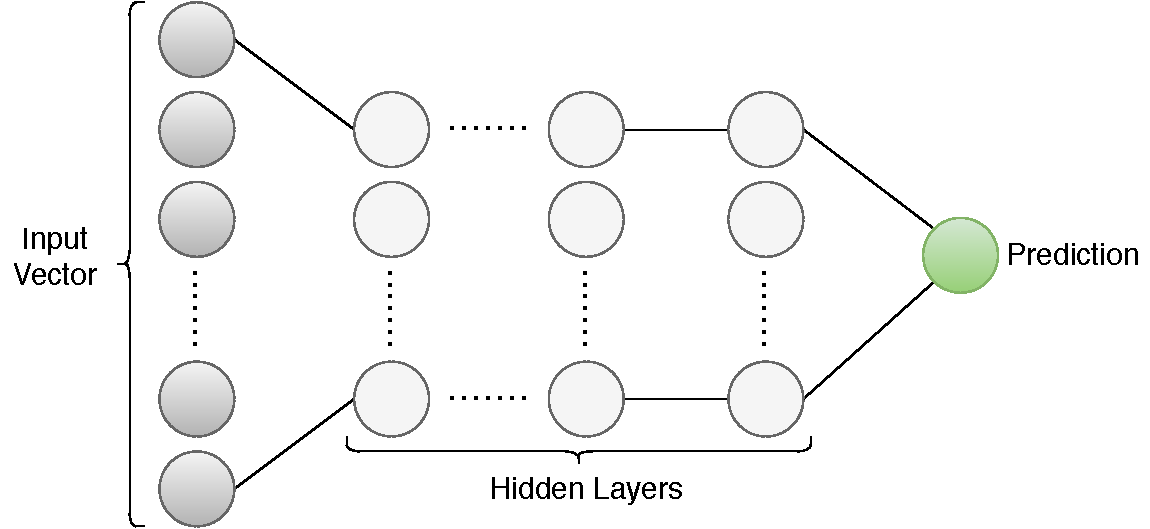
\includegraphics[clip,width=\columnwidth]{figures/ffnn.pdf}%
}
\qquad
\subfloat[Eager-Stopping Neural Network.]{%
  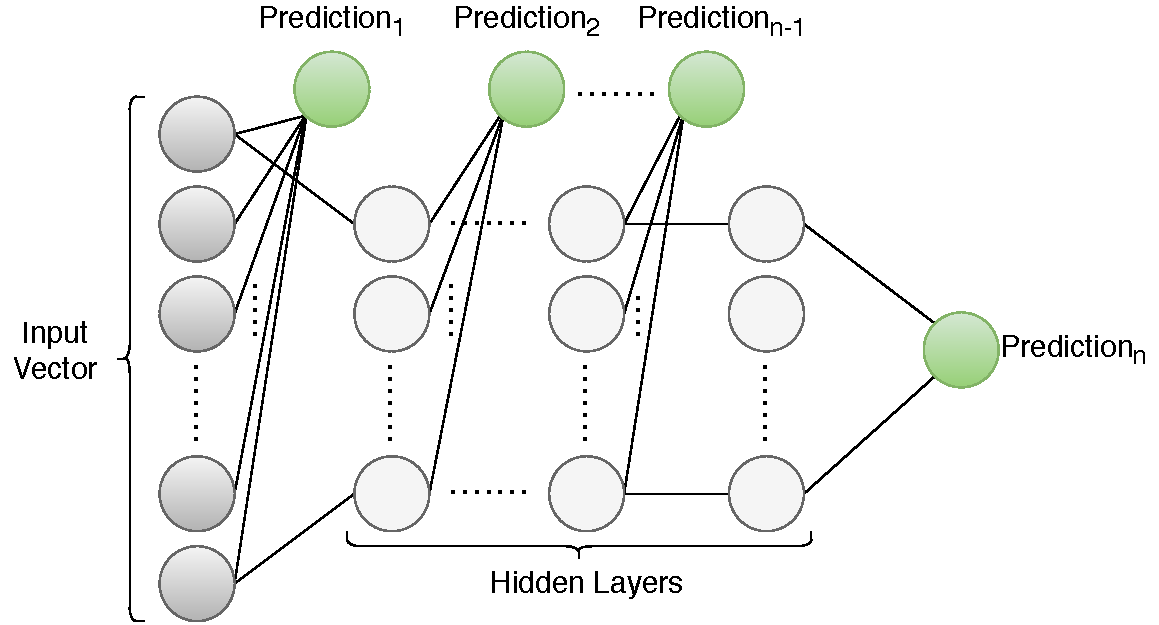
\includegraphics[clip,width=\columnwidth]{figures/eagernet.pdf}%
}

\caption{main caption}

\end{figure*}


\section{Related Work}

\section{Evaluation and Discussion}
\subsection{Datasets}

\begin{table}[ht!]
	
	\centering
	\caption{CAIA Flow Features.}
	\label{tab:cres}
	     
	\footnotesize
	\begin{tabular}{|c|c|c|}
		\toprule
		\textbf{Direction}                    & \textbf{Features}        & \textbf{Statistical Operations}        \\
		\midrule
		    
		                                      & flowDurationMilliseconds &                                        \\
		                                      & sourceTransportPort      &                                        \\
		                                      & destinationTransportPort &                                        \\
		                                      & protocolIdentifier       &                                        \\
		                                      & octetTotalCount          &                                        \\
		\midrule
		\multirow{7}{*}{Forward and Backward} & ipTotalLength            & \multirow{2}{*}{Mean, Min, Max, Stdev} \\
		                                      & interPacketTimeSeconds   &                                        \\
		\cmidrule{2-3}
		                                      & packetTotalCount         &                                        \\
		                                      & tcpSynTotalCount         &                                        \\
		                                      & tcpAckTotalCount         &                                        \\
		                                      & tcpFinTotalCount         &                                        \\
		                                      & tcpCwrTotalCount         &                                        \\
		   
		\midrule
		
		
	\end{tabular}
		
\end{table}

\subsection{Binary vs. Multiclass Classification}

\begin{table*}
\parbox{.45\linewidth}{
\centering
\begin{tabular}{cccrrrr}
\toprule
\textbf{Variant} & \textbf{Weights} & \textbf{Layers} & \textbf{Acc.} & \textbf{Prec.} & \textbf{Rec.} & \textbf{J.}\\
\midrule
\multirow{6}{*}{\rotatebox{90}{Binary}} & \multirow{2}{*}{Equal} & 1-3-1 & & & & \\
 & & 1-1-1 & & & & \\
 & \multirow{2}{*}{Increasing} & 1-3-1 & & & & \\
 & & 1-1-1 & & & & \\
 & \multirow{2}{*}{Decreasing} & 1-3-1 & & & & \\
 & & 1-1-1 & & & & \\
\midrule
\multirow{6}{*}{\rotatebox{90}{Multiclass}} & \multirow{2}{*}{Equal} & 1-3-1 & & & & \\
 & & 1-1-1 & & & & \\
 & \multirow{2}{*}{Increasing} & 1-3-1 & & & & \\
 & & 1-1-1 & & & & \\
 & \multirow{2}{*}{Decreasing} & 1-3-1 & & & & \\
 & & 1-1-1 & & & & \\
\end{tabular}
\caption{CIC-IDS17}
}
\hfill
\parbox{.45\linewidth}{
\centering
\begin{tabular}{cccrrrr}
\toprule
\textbf{Variant} & \textbf{Weights} & \textbf{Layers} & \textbf{Acc.} & \textbf{Prec.} & \textbf{Rec.} & \textbf{J.}\\
\midrule
\multirow{6}{*}{\rotatebox{90}{Binary}} & \multirow{2}{*}{Equal} & 1-3-1 & & & & \\
 & & 1-1-1 & & & & \\
 & \multirow{2}{*}{Increasing} & 1-3-1 & & & & \\
 & & 1-1-1 & & & & \\
 & \multirow{2}{*}{Decreasing} & 1-3-1 & & & & \\
 & & 1-1-1 & & & & \\
\midrule
\multirow{6}{*}{\rotatebox{90}{Multiclass}} & \multirow{2}{*}{Equal} & 1-3-1 & & & & \\
 & & 1-1-1 & & & & \\
 & \multirow{2}{*}{Increasing} & 1-3-1 & & & & \\
 & & 1-1-1 & & & & \\
 & \multirow{2}{*}{Decreasing} & 1-3-1 & & & & \\
 & & 1-1-1 & & & & \\
\end{tabular}
\caption{UNSW-NB15}
}
\end{table*}

\section{Conclusion}


\section*{Acknowledgements}
The Titan Xp used for this research was donated by the NVIDIA Corporation.

\bibliographystyle{ACM-Reference-Format}
\bibliography{bibliography}

\end{document}
